\chapter{Performance Analysis}\label{cap:rendimiento}
\noindent In this chapter qosh performance will be evaluated deployed over a real cluster. The execution environment will be described first and the metrics collected will be analyzed and put in context thereafter.

\section{Testing Environment}\label{sec:entornodeprueba}
\noindent Figure \ref{fig:clusterdespliegue} shows how the cluster is configured. The leftmost part of the figure shows the Cloud Controller; the rightmost, the Cloud Node. The Cloud Controller has been put through a full OpenStack Folsom installation --- except for Cinder, Swift or Quantum as they will not used ---, plus MySQL, Fabric and Qpid as message broker. In the Cloud Node only the bare minimum to support VM execution has been installed --- OpenStack Compute. The other required \emph{amenities} of the Cloud Node are delegated to the Controller via Qpid.

\begin{figure}[tbp]
\begin{center}
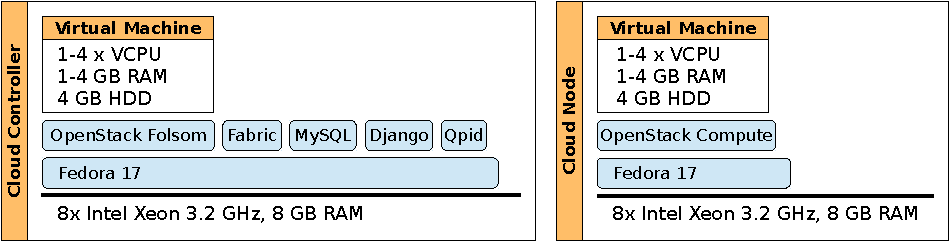
\includegraphics[width=0.99\textwidth]{imagenes/038.pdf}
 \caption{Deployment morphology}
\label{fig:clusterdespliegue}
\end{center}
\end{figure}

Regarding the physical layer, both nodes posses the same hardware configuration: Octa core Intel Xeon processor @ 3.2 \emph{GHz} with VT-x, 8 GB of RAM, 200 GB SATA 3 Gb/s 7200 RPM and Gigabit networking interface.

The Hadoop virtual image, whose creation procedure is described in section \ref{subsec:maquinavirtual}, will be used to create the VM instances that will effectively carry out the computations. Hadoop version is 1.0.4 and JRE's is 1.7v6 from Oracle. Figure \ref{fig:clusterdespliegue} shows the Hadoop VM in context. This instance will be increasingly provided from 1 to 4 GB of RAM and the same number of VCPUs to assess qosh's scaling. This varying amount of RAM will be shared between the guest OS and the JVM. The deployment has been configured to allow Hadoop to address all the memory in the VM --- except for those addresses in use by the OS and the JVM.

\section{Testing Methodology}\label{sec:metodologiaprueba}
\noindent This section contains both in and out scalability analysis and a study on the behavior on increasing input sizes. To evaluate how qosh scales, a map reduce work flow, large enough to stress every instance in the virtual cluster, will be fed to Hadoop; the work flow will count the words in 62.5 MB of plain text.

To actually assess the horizontal scalability, the size of the virtual cluster will progressively be doubled starting from one instance up to four. To test vertical scalability, two VMs will be initially spawned with 1 GB of RAM each, to have their RAM and VCPU count doubled on each test case until reaching 4 GB. Finally, to evaluate running time tendency input text size will be doubled from the original 62.5 MB to 250 MB.

As Glance and Compute cooperate to cache images, the time required to start an instance of some image will be longer the first time it launches, effectively skewing results. To get rid of those divergences, the instances on each flavor will be \textbf{warmed} by starting and destroying them before taking measures.



A priori, la variabilidad esperada de los resultados entre ejecuciones es lo suficientemente peque\~na como para fijar a \emph{diez} el n\'umero de realizaciones de cada caso de prueba ---esta suposici\'on a priori se ve confirmada a posteriori a la vista del resultado de los experimentos. Para ello se har\'an medidas auto\-ma\-ti\-za\-das, con marcas de tiempo directamente en el c\'odigo, que distinguir\'an los siguientes cinco tiempos de inter\'es:

\begin{description}
    \item[Despliegue:] tiempo transcurrido desde que se hace la petici\'on \emph{crear ins\-tan\-cia} hasta que se puede acceder a todas ellas.
  \item[Configuraci\'on:] tiempo necesario para que se establezca el marco de ejecuci\'on para Hadoop. Incluye el tiempo de transferencia y descompresi\'on de los datos de entrada a la m\'aquina virtual y a HDFS, y la configuraci\'on del cl\'uster virtual Hadoop conformado por todas las instancias creadas.
  \item[MapReduce:] tiempo dedicado por Hadoop a la ejecuci\'on del trabajo wordcount.
  \item[Borrado:] tiempo utilizado para limpiar el entorno de ejecuci\'on. No incluye el tiempo requerido por OpenStack para eliminar por completo las ins\-tan\-cias.
  \item[Total:] tiempo que transcurre desde que se inicia el despliegue hasta que finaliza la petici\'on de borrado de las instancias.
\end{description}

Notar que los resultados presentados hacen referencia a la media aritm\'etica de las diez ejecuciones para cada caso. 


\section{An\'alisis de resultados}\label{sec:analisisresultados}

\begin{figure}[tbp]
\begin{center}
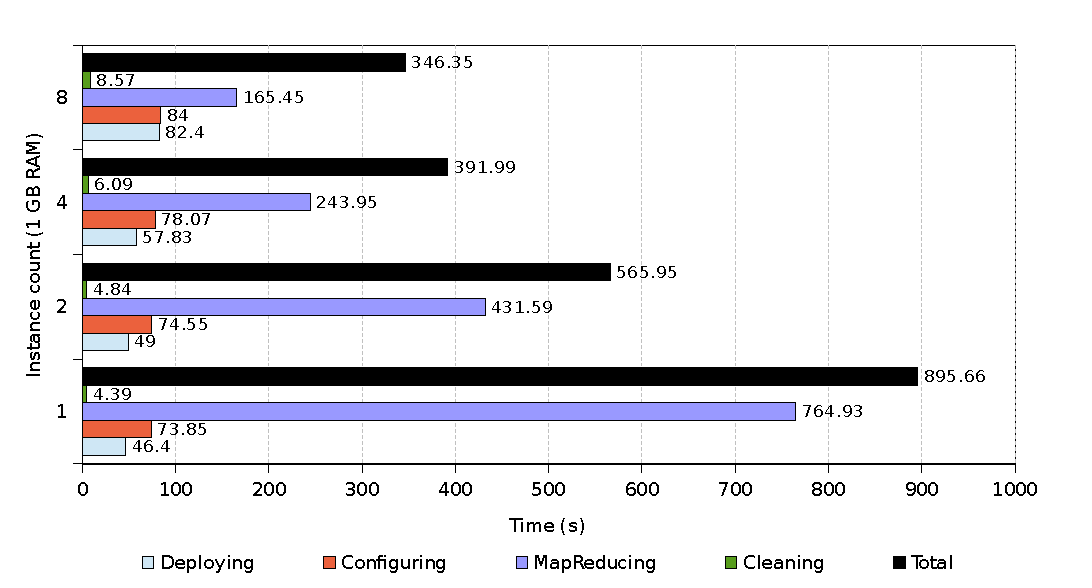
\includegraphics[width=0.98\textwidth]{imagenes/039.pdf}
\caption{Escalabilidad horizontal}
\label{fig:eschorizontal}
\end{center}
\end{figure}

\noindent La figura \ref{fig:eschorizontal} presenta la evoluci\'on de los distintos tiempos de inter\'es en funci\'on del n\'umero de instancias creadas, desde una hasta ocho. \newline

En ella se observa que los tiempos de despliegue, configuraci\'on y borrado aumentan ligeramente con el n\'umero de instancias desplegadas, mientras el tiempo de procesamiento se ve reducido. Esto es, el despliegue, la con\-fi\-gu\-ra\-ci\'on y el borrado dependen solamente del tama\~no del cl\'uster virtual; por el contrario, el tiempo MapReduce ---y por lo tanto tambi\'en el tiempo total--- depende adem\'as del volumen del trabajo a ejecutar. La figura \ref{fig:escvertical} presenta la evoluci\'on de los cinco tiempos de inter\'es a medida que se aumentan la cantidad de RAM y las CPUs virtuales de las dos instancias creadas; desde 1 GB y 1 VCPU hasta 4. \newline

\begin{figure}[tbp]
\begin{center}
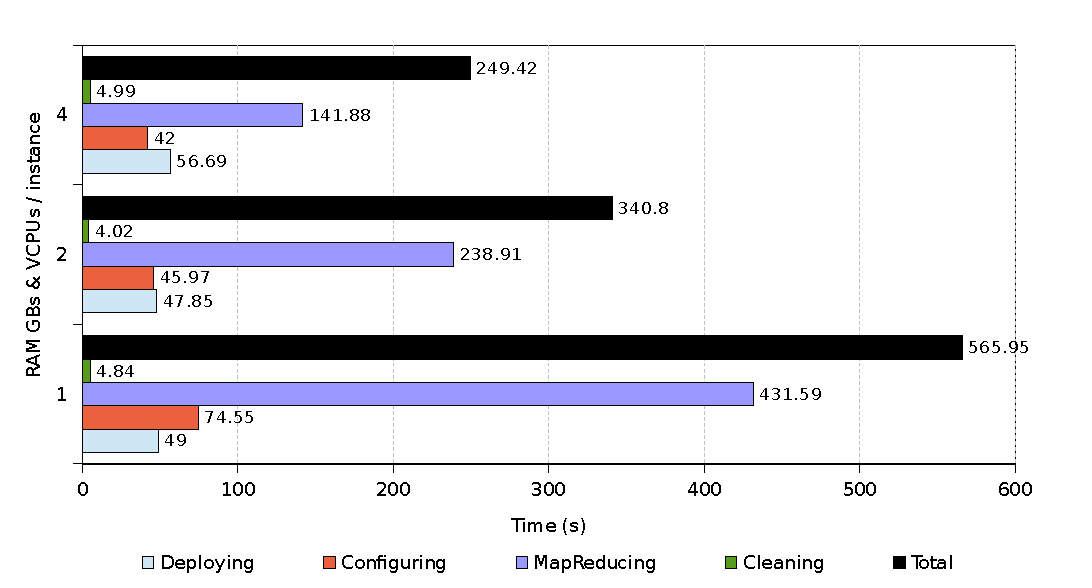
\includegraphics[width=0.98\textwidth]{imagenes/041.pdf}
\caption{Escalabilidad vertical}
\label{fig:escvertical}
\end{center}
\end{figure}

A la vista de esta figura, tal vez lo m\'as llamativo sean los tiempos de des\-plie\-gue y borrado, pudiendo considerarse pr\'acticamente constantes a pesar de aumentar la capacidad de c\'alculo de las instancias. Dicho de otro modo, la dificultad que supone desplegar o borrar un cl\'uster virtual en nuestro entorno depende exclusivamente del n\'umero de instancias o nodos virtuales ---conclusi\'on que ya hab\'iamos alcanzado previamente. Precisamente, hab\'iamos observado c\'omo la complejidad de configuraci\'on crec\'ia proporcionalmente con el tama\~no del cl\'uster. En este caso sucede lo contrario: al estar mejorando las caracter\'isticas t\'ecnicas de las dos instancias, los tiempos de configuraci\'on de Hadoop se ven l\'ogicamente reducidos. Es decir, la conclusi\'on revisada dicta que el tiempo de configuraci\'on var\'ia de forma directa con el n\'umero de instancias y de forma inversa con las capacidades operativas de las mismas. \newline

Los resultados contenidos en estas gr\'aficas demuestran que nuestra soluci\'on se comporta de modo m\'as eficaz cuando se mejora la capacidad de c\'omputo de las instancias ---escalabilidad vertical--- en vez de aumentar el tama\~no del cl\'uster virtual soporte ---escalabilidad horizontal. Este hecho se observa con claridad en las figuras \ref{fig:eschorizontal} y \ref{fig:escvertical} al comparar los casos extremos de prueba: ocho instancias de 1 GB de RAM frente a 4 GB de RAM y VCPUs por ins\-tan\-cia, respectivamente. Ambos casos distribuyen sendos clusters virtuales con las mismas caracter\'isticas de 8 VCPUs y 8 GB de RAM sobre nuestros nodos de prueba. Sin embargo, el tiempo de ejecuci\'on total es casi un \texttt{28\%} menor al mejorar las dos instancias (figura \ref{fig:escvertical}); esperable, en cierta medida, al ahorrar la sobrecarga de comunicaci\'on por la red. \newline

\begin{figure}[tbp]
\begin{center}
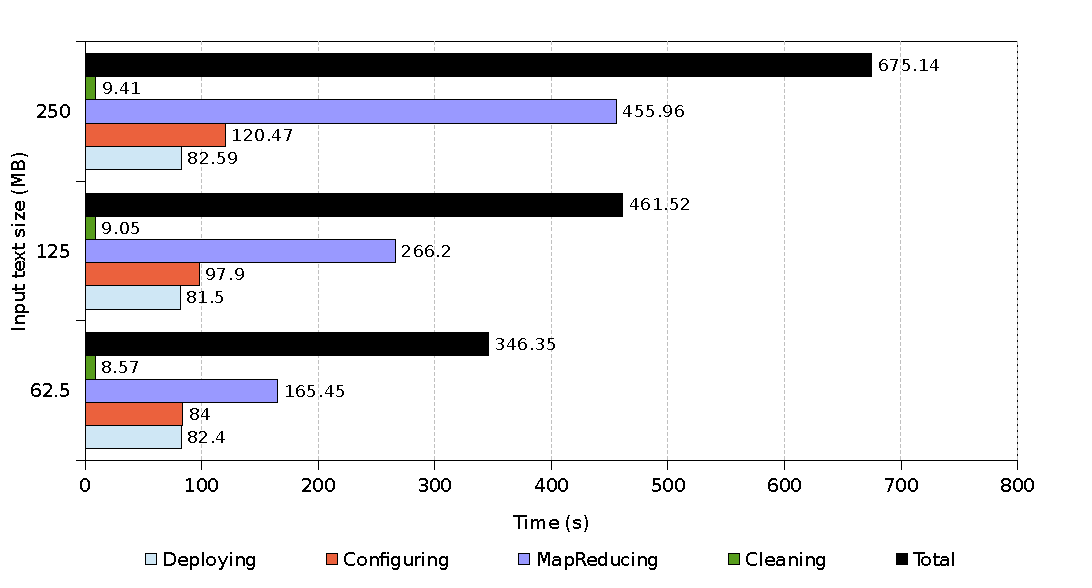
\includegraphics[width=0.98\textwidth]{imagenes/042.pdf}
\caption{Tama\~no de entrada frente a tiempo de ejecuci\'on}
\label{fig:evotemporal}
\end{center}
\end{figure}

La figura \ref{fig:evotemporal} muestra la evoluci\'on de los tiempos de ejecuci\'on al incrementar la magnitud de los datos a procesar. Como era de esperar, la duraci\'on de la etapa MapReduce y la duraci\'on total crecen en relaci\'on directa con el tama\~no de entrada, pero en menor medida. Los tiempos de despliegue y bo\-rra\-do se mantienen pr\'acticamente constantes en cada caso, mientras que el tiempo de configuraci\'on crece ligeramente, al englobar la descompresi\'on y posterior distribuci\'on de los ficheros de entrada sobre el cl\'uster Hadoop.
